\documentclass[../notebook.tex]{subfiles}

% \let\erf{\mathop\mathrm{erf}}

\begin{document}
\nbentry{July 5, 2020}{%
  Entropy of coordinate systems
}

What is the entropy of a continuous space, and what role does the choice of
coordinates play? We would like to capture the sense in which it takes much less
information to specify a point from a normal distribution with variance
$\sigma^2$ on $\RR^3$ than it does to specify an arbitrary point. Consider a
ball of radius $R$ about the origin. If $R \ll \sigma$, then both distributions
are about the same, and should not differ much in required information, but for
$R \gg \sigma$, the divergence of the uniform distribution from the normal
distribution should grow without bound.

Spherical coordinates are given by the usual map $\Phi:[0,R] \times [0,\pi]
\times [0,2\pi] \to \RR^3$ with Jacobian $r^2 \sin\theta$. A probability
distribution on $\RR^3$ may be pulled back to particular coordinates. The
uniform distribution on the ball $B(\vb{0},\, R)$ pulls back on Cartesian
coordinates to
\[
  p_u(x,\, y,\, z)
  = \frac{3}{4\pi R^3},
\]
but on spherical coordinates pulls back to
\[
  p_u(r,\, \theta,\, \varphi)
  = \frac{3r^2 \sin\theta}{4\pi R^3}.
\]
The spherical coordinates form independent random variables with marginal
distributions
\[
  p_u(r)
  = \frac{3r^2}{R^3} \qc
  p_u(\theta)
  = \frac{\sin\theta}{2}, \qand
  p_u(\varphi)
  = \frac{1}{2\pi},
\]
whereas the Cartesian coordinates form dependent random variables with
conditional distributions
\[
  p_u(x_i \mathbin{|} x_{j \ne i})
  = \frac{1}{2}{\qty(R^2 - \sum_{j \ne i} x_j^2)}^{-1/2}.
\]
Similarly, the truncated normal distribution with unit variance on the ball
pulls back in spherical coordinates to
\[
  p(r,\, \theta,\, \varphi)
  = {\qty[\mathop{\mathrm{erf}}\qty(\frac{R}{\sqrt{2}})
  - R\sqrt{\frac{2}{\pi}}e^{-R^2 / 2}]}^{-1}
  \frac{e^{-r^2 / 2}}{\sqrt{8\pi^3}}\, r^2 \sin\theta.
\]
While $p(\theta) = p_u(\theta)$ and $p(\varphi) = p_u(\varphi)$, the marginal
distribution of the radius is
\[
  p(r)
  = {\qty[\mathop{\mathrm{erf}}\qty(\frac{R}{\sqrt{2}})
  - R\sqrt{\frac{2}{\pi}}e^{-R^2 / 2}]}^{-1}
  \frac{e^{-r^2 / 2}}{\sqrt{2\pi}}\, 2r^2.
\]
The KL divergence from the uniform to the truncated normal distribution over the
ball is
\[
  D_{KL}(p \mathbin\| p_u)
  = \int_{r=0}^R \int_{\theta=0}^\pi \int_{\varphi=0}^{2\pi} p \ln
  \frac{p}{p_u} \dd{r}\dd{\theta}\dd{\varphi},
\]
independent of using spherical coordinates
(Fig.~\ref{fig:trunc-norm-ball-kldiv}). But since the spherical coordinates form
independent random variables for both distributions, this separates as
\begin{align}
  &D_{KL}(p(r,\, \theta,\, \varphi) \mathbin\| p_u(r,\, \theta,\, \varphi)) \\
  &= D_{KL}(p(r) \mathbin\| p_u(r))
  + D_{KL}(p(\theta) \mathbin\| p_u(\theta))
  + D_{KL}(p(\varphi) \mathbin\| p_u(\varphi)).
\end{align}
As only the radial distribution is different,
\[
  D_{KL}(p(r,\, \theta,\, \varphi) \mathbin\| p_u(r,\, \theta,\, \varphi))
  = D_{KL}(p(r) \mathbin\| p_u(r)),
\]
as expected from the symmetries.

\begin{figure}[h]
  \centering
  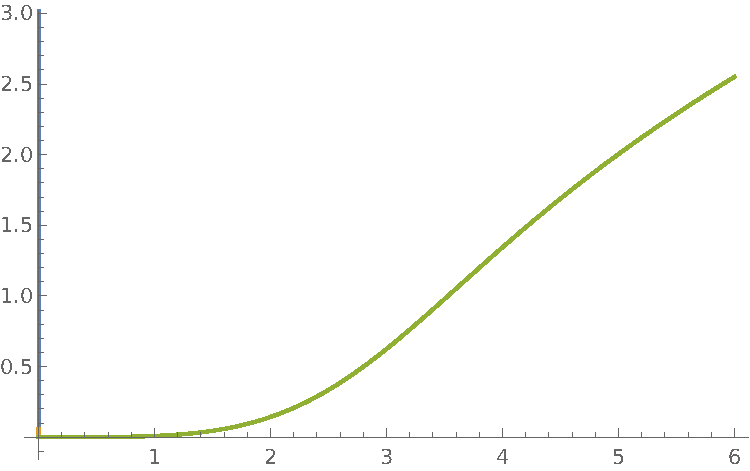
\includegraphics[width=0.9\linewidth]{trunc-norm-ball-kldiv}
  \caption{The KL divergence from uniform to truncated normal as a function of
  ball radius.}\label{fig:trunc-norm-ball-kldiv}
\end{figure}

How can we quantify the relative information between coordinates $(x_1,\,
\ldots,\, x_m)$? I suggest
\[
  I(x_i)
  = \frac{D_{KL}(p(x_i) \mathbin\| p_u(x_i))}{%
  D_{KL}(p(x_1,\, \ldots,\, x_m) \mathbin\| p_u(x_1,\, \ldots,\, x_m))}
\]
as a measure of the information in the coordinate $x_i$ given the distribution
$p$. This is relative to the uniform distribution $p_u$ where all coordinates
are considered equally informative, but a different reference distribution may
be chosen for unbounded parameters. This quantity is invariant under changes in
scale and has $\sum_i I(x_i) = 1$.

A simple example is a uniform distribution on a rectangle. The idea is that to
determine a point in a square within the rectangle, it helps more to know the
coordinate of the longer side. To encode this in probability distributions, we
let $p_u(x,\, y) = {(ab)}^{-1} [0 \le x \le a,\, 0 \le y \le b]$ and $p(x,\, y)
= c^{-2} [0 \le x \le c,\, 0 \le y \le c]$ with $c \le a \le b$. Then
\[
  I(x)
  = \frac{D_{KL}(p(x) \mathbin\| p_u(x))}{%
  D_{KL}(p(x,\, y) \mathbin\| p_u(x,\, y))}
  = \frac{\ln(a/c)}{\ln(a/c) + \ln(b/c)},
\]
with $I(y)$ defined similarly. As $c \to 0$, $I \to 1/2$, as the dimensions of
the rectangle become irrelevant. As $c \to a$, $I(x) \to 0$ and $I(y) \to 1$, as
you only need to restrict $y$ for a point to be in the square. If $a = b$, then
there is never any difference and $I(x) = I(y) = 1/2$ independent of $c$. For $a
\ll b$, $I(x)$ is nearly zero and $I(y)$ is nearly one over most of the range of
$c$, though both still return to $1/2$ as $c \to 0$.

In light of the previous calculation in spherical coordinates, we see that $I(r)
= 1$ and $I(\theta) = I(\varphi) = 0$, since we need only know the radius to
know if a point is probable.

\end{document}

